\documentclass[12pt]{scrartcl}
\usepackage{tikz}
\usepackage{amssymb}
\usetikzlibrary{positioning}
\usetikzlibrary{calc}
\usetikzlibrary{arrows,shapes,snakes,automata,petri}


\begin{document}
	
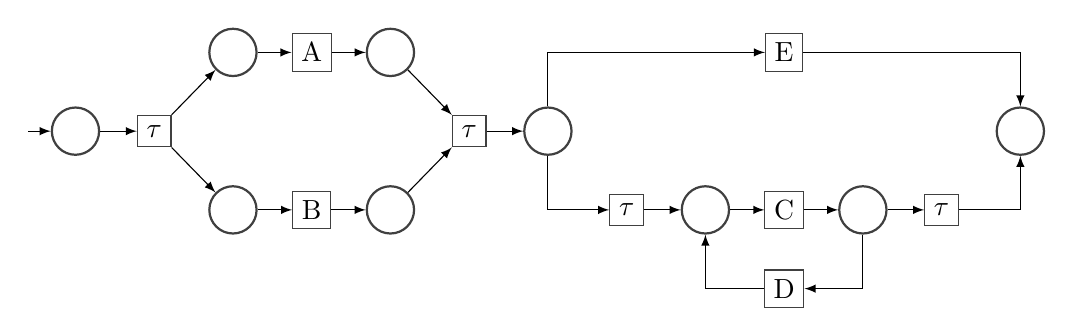
\begin{tikzpicture}
\tikzstyle{place} =[circle,thick,draw=black!75,minimum size=6mm]
\tikzstyle{transition} =[rectangle,draw=black!75,minimum size=4mm]
\node[place](init) at (0, 0) {};
\draw[draw,-latex]($(init)+(-0.6,0)$)--(init.west);
\node[place](preA) at ($(init)+(2,1)$){};
\node[place](preB) at ($(init)+(2,-1)$){};
\node[place](postA) at ($(init)+(4,1)$){};
\node[place](postB) at ($(init)+(4,-1)$){};
\node[place](postinv2) at ($(init)+(6,0)$){};
%\node[place](postE) at ($(init)+(9,1)$){}; 
\node[place](postinv3) at ($(init)+(8,-1)$){};
\node[place](postC) at ($(init)+(10,-1)$){};
\node[place](end) at ($(init)+(12,0)$){};

\node[transition](inv1) at ($(init)+(1,0)$){$\tau$};
\draw[draw,-latex] (init.east)--(inv1.west);
\draw[draw,-latex] (inv1.north east)--(preA.south west);
\draw[draw,-latex] (inv1.south east)--(preB.north west);

\node[transition](A) at ($(init)+(3,1)$){A};
\draw[draw,-latex] (preA.east)--(A.west);
\draw[draw,-latex] (A.east)--(postA.west);

\node[transition](B) at ($(init)+(3,-1)$){B};
\draw[draw,-latex] (preB.east)--(B.west);
\draw[draw,-latex] (B.east)--(postB.west);

\node[transition](inv2) at ($(init)+(5,0)$){$\tau$};
\draw[draw,-latex] (postA.south east)--(inv2.north west);
\draw[draw,-latex] (postB.north east)--(inv2.south west);
\draw[draw,-latex] (inv2.east)--(postinv2.west);

\node[transition](E) at ($(init)+(9,1)$){E};
\draw[draw] (E.east)--($(init)+(12,1)$);
\draw[draw,-latex] ($(init)+(12,1)$)--(end.north);

\node[transition](inv3) at ($(init)+(7,-1)$){$\tau$};
\draw[draw,-latex] (inv3.east)--(postinv3.west);

\draw[draw,] (postinv2.north)--($(init)+(6,1)$);
\draw[draw,-latex] ($(init)+(6,1)$)--(E.west);

\draw[draw](postinv2.south)--($(init)+(6,-1)$);
\draw[draw,-latex]($(init)+(6,-1)$)--(inv3.west);

\node[transition](C) at ($(init)+(9,-1)$){C};
\draw[draw,-latex] (postinv3.east)--(C.west);
\draw[draw,-latex] (C.east)--(postC.west);

\node[transition](D) at ($(init)+(9,-2)$){D};
\draw[draw](postC.south)--($(init)+(10,-2)$);
\draw[draw,-latex]($(init)+(10,-2)$)--(D.east);
\draw[draw](D.west)--($(init)+(8,-2)$);
\draw[draw,-latex]($(init)+(8,-2)$)--(postinv3.south);

\node[transition](inv5) at ($(init)+(11,-1)$){$\tau$};
\draw[draw,-latex](postC.east)--(inv5.west);
\draw[draw] (inv5.east)--($(init)+(12,-1)$);
\draw[draw, -latex] ($(init)+(12,-1)$)--(end.south);
\end{tikzpicture}
\end{document}